\section{Modelagem do sistema}
\label{sec:modelling}
%===============================================================================

O objetivo da modelagem de um sistema � encontrar um modelo (fun��o com par�metros
livres) que consiga representar o sistema f�sico de forma completa. A partir do
conhecimento do sistema f�sico, fazem-se considera��es sobre o sistema, para simplifica-lo
a fim de tornar o modelo matem�tico o mais simples poss�vel, mas que ainda represente
o sistema real, com a margem de preciosidade definida, pela quantidade e qualidade 
das simplifica��es aplicadas para chegar-se ao modelo matem�tico do sistema.

\subsection{Sistema F�sico}
%===============================================================================

O sistema f�sico em estudo neste trabalho, � um sistema para controle de posi��o, onde 
o atuador � um motor de corrente continua (DC). Desta forma a entrada do sistema 
� a tens�o aplicada sobre os terminais do motor em Volts [V], e a sa�da � a posi��o
angular do motor em radianos [rad].

Na Figura (\ref{fig:motor_system}) pode ser vista a representac�o eletrica e mecanica
do motor em quest�o.

\begin{figure}[htbp]
	\center
	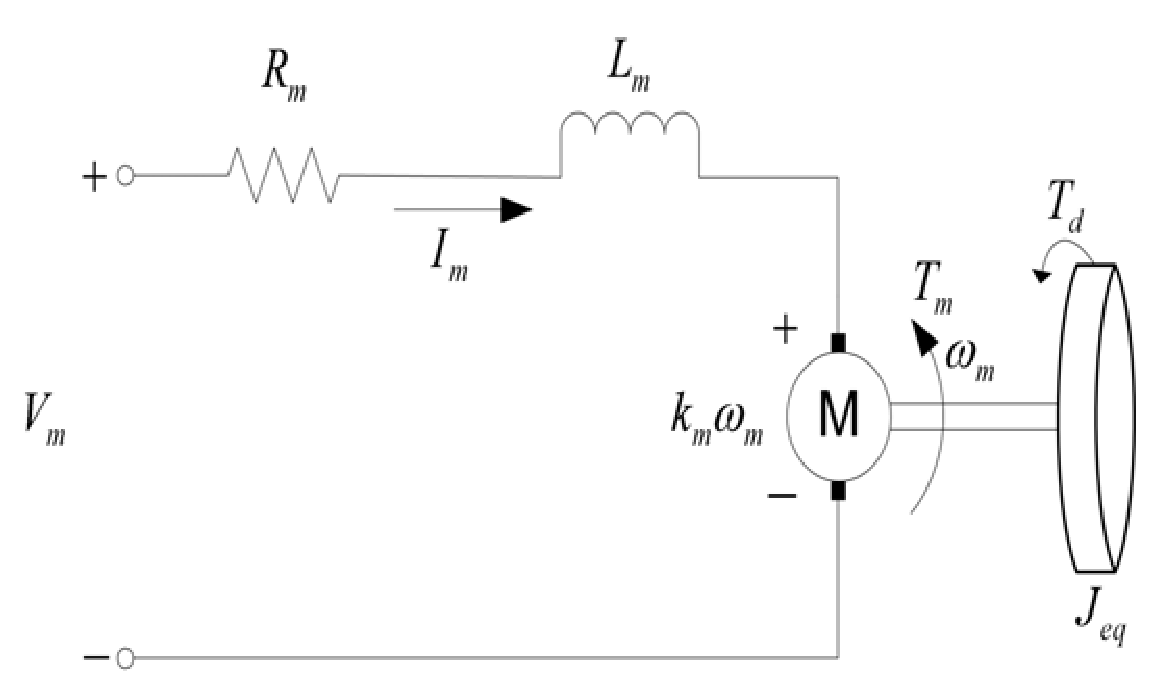
\includegraphics[width=0.7\columnwidth]{figures/motor_system.eps}
	\caption{TODO}
	\label{fig:motor_system}
\end{figure}

As vari�veis consideradas para a modelagem s�o as apresentadas abaixo:

\begin{itemize}
	\item $\omega$ = Velocidade do motor = vari�vel de sa�da.
	\item \it{v} = tens�o aplicada na armadura = vari�vel de entrada.
	\item \it{ia} = corrente de armadura.
	\item \it{L} = Indut�ncia da armadura = $10\mu H$
	\item \it{e} = Forca contra eletromotriz = $K_{2} \omega$
	\item \it{$K_{2}$} = $5.5x10^{-2} V.s/rad$ 
	\item \it{R} = Resist�ncia do enrolamento da armadura = $0.2 \Omega$
	\item \it{T} = Torque aplicado = $K_{i} ia$
	\item \it{$K_{1}$} = $6x10^{-5} Kg.m/A$
	\item \it{J} = Momento de inercia da carga = $4x10^{-3} Kg.m.s^{2}$
	\item \it{f} = Atrito viscoso no eixo = $4x10^{-2} Kg.m.s/rad$
\end{itemize}
